\section{Các objects khác}
\subsection{Nền trời}
Được tạo nên từ mặt bên trong của hình cầu với vật liệu là MeshPhongMaterial:
\begin{itemize}
    \item map: sử dụng texture nền bầu trời
    \item side:THREE.DoubleSide,
    \item shadowSide:THREE.DoubleSide 
\end{itemize}

\subsection{Nền đất}
Được tạo nên từ bề mặt bên ngoài của hình cầu với vật liệu là MeshStandardMaterial:
\begin{itemize}
    \item map: sử dụng texture nền thảm cỏ
    \item side:THREE.FrontSide
    \item transparent: false
    \item metalness:0
\end{itemize}

\begin{center}
    \begin{figure}[!h]
        \centering
        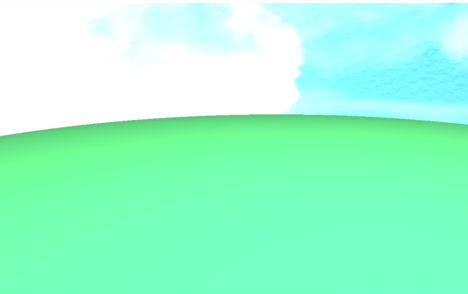
\includegraphics[scale = 1]{contents/day.png}
        \caption{Khung cảnh ngoài trời tạo bởi nền trời và đất}
    \end{figure}
\end{center}

\begin{center}
    \begin{figure}[!h]
        \centering
        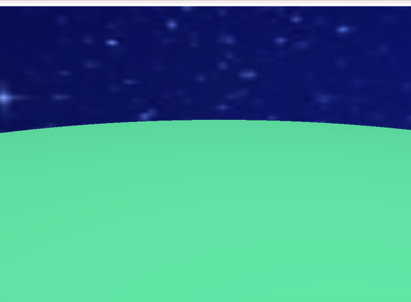
\includegraphics[scale = 1]{contents/night.png}
        \caption{Khung cảnh ngoài trời tạo bơi nền trời và đất}
    \end{figure}
\end{center}

\subsection{Hòn đá}
Được tạo nên từ hình cầu với vật liệu là MeshLambertMaterial:
\begin{itemize}
    \item color:"\#a0a0a0", 
     \item     side:THREE.DoubleSide,
    \item         shadowSide:THREE.DoubleSide
\end{itemize}


\subsection{Khung nhà}
Với khung cảnh trong nhà, do model được đọc vào chỉ là 1 góc nên để tạo độ chân thật cho khung cảnh này thì ở đây có vẽ thêm 1 cái hình hộp.\\

Hình hộp này có vật liệu là MeshLambertMaterial:
\begin{itemize}
    \item side:THREE.DoubleSide,
    \item shadowSide:THREE.DoubleSide
\end{itemize}
